\documentclass[tikz,border=8pt]{standalone}
% Estilos del modelo C4 para TikZ (colores y formas de C4). Los tres diagramas del informe los cargan con \input.
\usepackage{fontspec}
\usepackage{xcolor}
\usetikzlibrary{shapes.geometric,arrows.meta,positioning,calc,fit,backgrounds}
\renewcommand{\familydefault}{\sfdefault}
\hyphenpenalty=10000 \exhyphenpenalty=10000 % sin guiones al partir las palabras en las cajas

\definecolor{c4persona}{HTML}{08427B}   \definecolor{c4personab}{HTML}{073B6F}
\definecolor{c4sistema}{HTML}{1168BD}   \definecolor{c4sistemab}{HTML}{0B4884}
\definecolor{c4externo}{HTML}{999999}   \definecolor{c4externob}{HTML}{6B6B6B}
\definecolor{c4cont}{HTML}{438DD5}      \definecolor{c4contb}{HTML}{3C7FC0}
\definecolor{c4comp}{HTML}{85BBF0}      \definecolor{c4compb}{HTML}{78A8D8}

% \elem{Nombre}{[Tipo: tecnología]}{Descripción}: el texto de un elemento en tres líneas, como en C4.
\newcommand{\elem}[3]{\textbf{#1}\\[1pt]{\scriptsize #2}\if\relax\detokenize{#3}\relax\else\\[3pt]{\scriptsize #3}\fi}

\tikzset{
  c4box/.style={draw, rounded corners=4pt, align=center, inner sep=5pt, text=white, font=\sffamily\small,
                text width=3.1cm, minimum height=2.0cm},
  persona/.style={c4box, fill=c4persona, draw=c4personab},
  sistema/.style={c4box, fill=c4sistema, draw=c4sistemab},
  externo/.style={c4box, fill=c4externo, draw=c4externob},
  contenedor/.style={c4box, fill=c4cont, draw=c4contb},
  componente/.style={c4box, fill=c4comp, draw=c4compb, text=black},
  basedatos/.style={contenedor, shape=cylinder, shape border rotate=90, aspect=0.16, minimum height=2.4cm},
  limite/.style={draw=c4externob, dashed, rounded corners=6pt, inner sep=0.45cm},
  rel/.style={-{Stealth[length=2.4mm,width=1.9mm]}, line width=0.7pt, color=black!70},
  etq/.style={fill=white, inner sep=1.5pt, align=center, font=\sffamily\scriptsize, text=black!85},
}

% Cabeza de una persona (se dibuja detrás de su caja): \cabeza{nombre de la caja}
\newcommand{\cabeza}[1]{\begin{scope}[on background layer]\node[circle, fill=c4persona, draw=c4personab, minimum size=0.9cm] at ([yshift=0.18cm]#1.north) {};\end{scope}}

\begin{document}
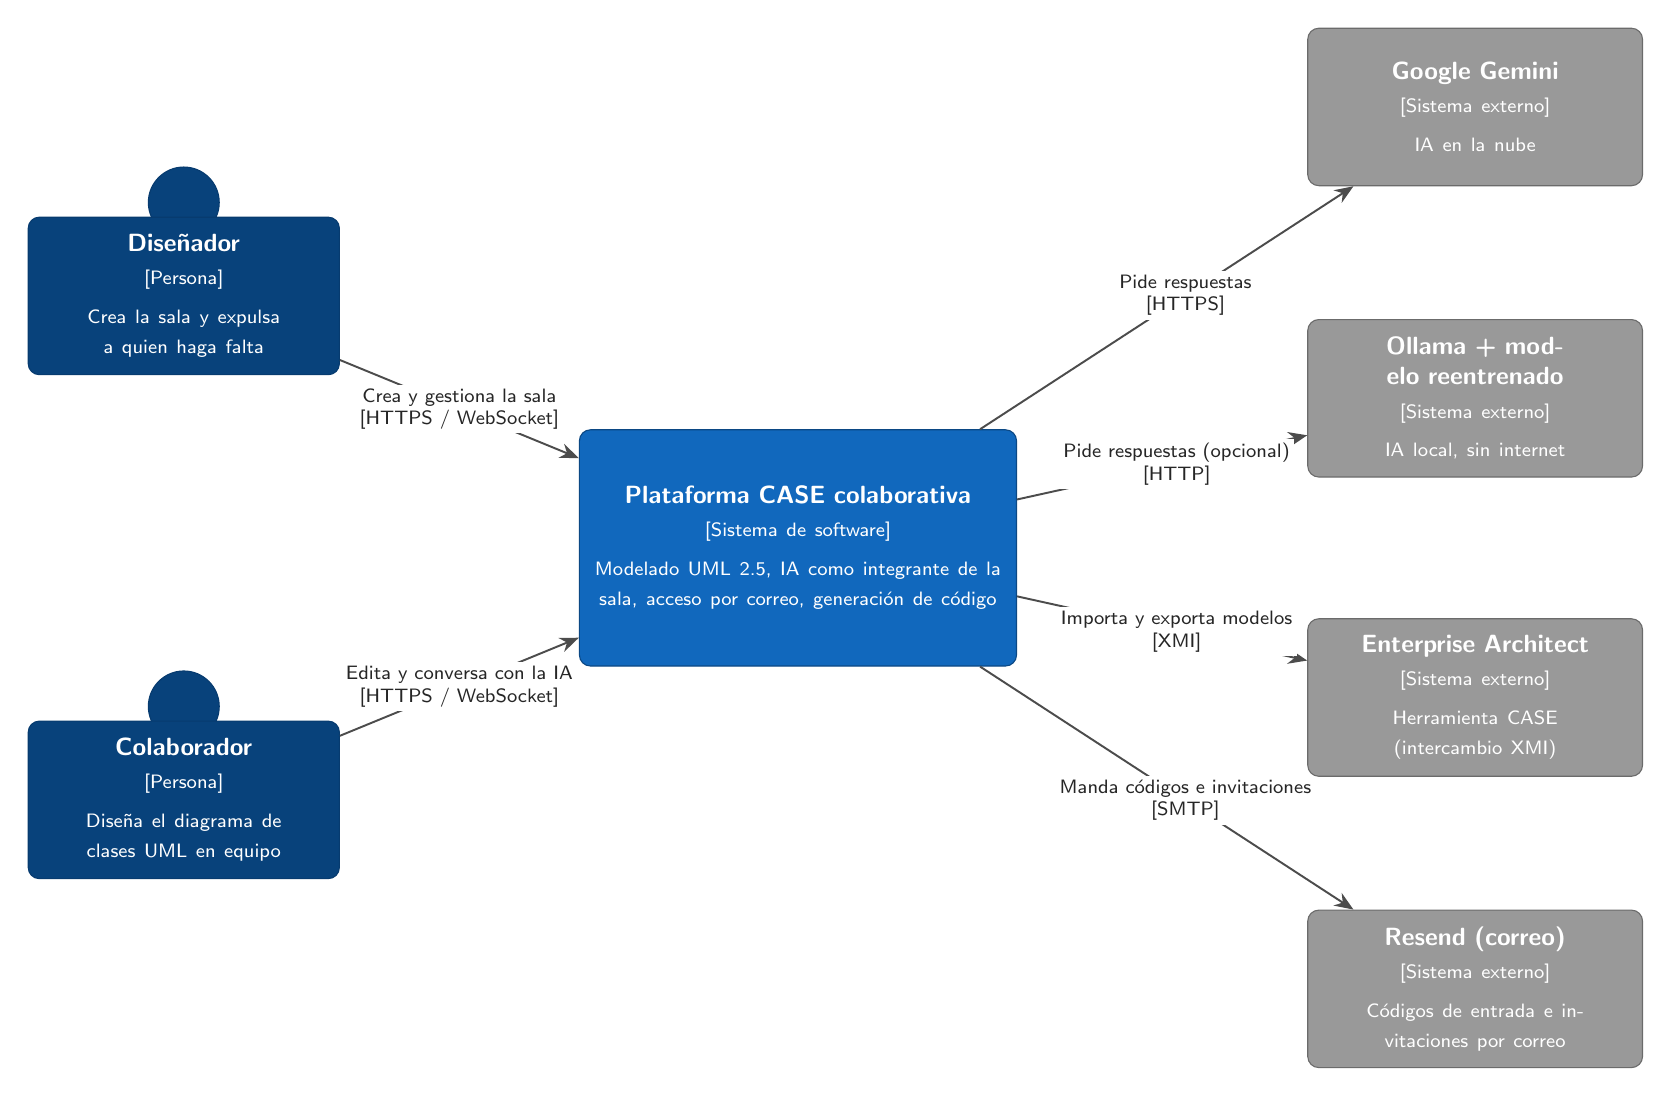
\begin{tikzpicture}
  % personas a la izquierda, el sistema en el centro y los sistemas externos a la derecha
  \node[persona, text width=3.6cm] (p1) at (0, 3.2) {\elem{Diseñador}{[Persona]}{Crea la sala y expulsa a quien haga falta}};
  \node[persona, text width=3.6cm] (p2) at (0,-3.2) {\elem{Colaborador}{[Persona]}{Diseña el diagrama de clases UML en equipo}};
  \cabeza{p1} \cabeza{p2}
  \node[sistema, text width=5.2cm, minimum height=3.0cm] (s) at (7.8, 0) {\elem{Plataforma CASE colaborativa}{[Sistema de software]}{Modelado UML 2.5, IA como integrante de la sala, acceso por correo, generación de código}};
  \node[externo, text width=3.9cm] (g) at (16.4, 5.6) {\elem{Google Gemini}{[Sistema externo]}{IA en la nube}};
  \node[externo, text width=3.9cm] (o) at (16.4, 1.9) {\elem{Ollama + modelo reentrenado}{[Sistema externo]}{IA local, sin internet}};
  \node[externo, text width=3.9cm] (e) at (16.4,-1.9) {\elem{Enterprise Architect}{[Sistema externo]}{Herramienta CASE (intercambio XMI)}};
  \node[externo, text width=3.9cm] (m) at (16.4,-5.6) {\elem{Resend (correo)}{[Sistema externo]}{Códigos de entrada e invitaciones por correo}};

  \draw[rel] (p1) -- node[etq, pos=0.5] {Crea y gestiona la sala\\{[HTTPS / WebSocket]}} (s);
  \draw[rel] (p2) -- node[etq, pos=0.5] {Edita y conversa con la IA\\{[HTTPS / WebSocket]}} (s);
  \draw[rel] (s) -- node[etq, pos=0.55] {Pide respuestas\\{[HTTPS]}} (g);
  \draw[rel] (s) -- node[etq, pos=0.55] {Pide respuestas (opcional)\\{[HTTP]}} (o);
  \draw[rel] (s) -- node[etq, pos=0.55] {Importa y exporta modelos\\{[XMI]}} (e);
  \draw[rel] (s) -- node[etq, pos=0.55] {Manda códigos e invitaciones\\{[SMTP]}} (m);
\end{tikzpicture}
\end{document}
